\documentclass{sig-alternate}
%\documentclass[a4paper,10pt]{article}
\usepackage[utf8]{inputenc}
%El template pincha con spanish babel
%\usepackage[spanish]{babel}
\usepackage{amsmath, amssymb, amsfonts}
\usepackage{graphicx}
\usepackage{fancybox}
\usepackage[table]{xcolor}
\usepackage{soul}

\newtheorem{theorem}{Teorema}

\title{Que bien que est\'a esa cola} 

\numberofauthors{4}
\author{
\alignauthor
Pose, Alberto Miguel\\
       \affaddr{Instituto Tecnol\'ogico de Buenos Aires}\\
       \affaddr{Buenos Aires, Argentina}\\
       \email{apose@alu.itba.edu.ar}
\alignauthor
Catalano, Juan Ignacio\\
       \affaddr{Instituto Tecnol\'ogico de Buenos Aires}\\
       \affaddr{Buenos Aires, Argentina}\\
       \email{jcatalan@alu.itba.edu.ar}
\and
\alignauthor 
Palombo, Mart\'in\\
       \affaddr{Instituto Tecnol\'ogico de Buenos Aires}\\
       \affaddr{Buenos Aires, Argentina}\\
       \email{mpalombo@alu.itba.edu.ar}
\alignauthor 
V\'azquez, Santiago Jos\'e\\
       \affaddr{Instituto Tecnol\'ogico de Buenos Aires}\\
       \affaddr{Buenos Aires, Argentina}\\
       \email{savazque@alu.itba.edu.ar}
}

\date{}

\begin{document}

\maketitle

\begin{abstract}
Se estudia el modelo de cola M/M/1 y M/M/2. Se analizan los tiempos
medios de espera en la cola y la longitud de la misma.
\end{abstract}

\newpage

\section{Introducci\'on}

Se analiza el modelo de Cola simple mediante la simulaci\'on por eventos discretos.
La estructura din\'amica de dicha cola se la indica como M/M/$n$/$\infty$/FIFO, o simplemente M/M/$n$.
La M proviene de Markoviano, es decir, los tiempos entre llegadas y entre servicios son variables
aleatorias con distribuci\'on exponencial y los n\'umeros de llegadas y servicios en un cierto
intervalo de tiempo son procesos de Poisson.  Existen $n$ servidores que atiende a los clientes
y pueden haber infinitos de los mismos en la cola. Adem\'as, ocurre que el primer cliente en llegar es el primero en irse.
En este modelo, se asume que los clientes llegan al sistema mediante un proceso de Poisson con una tasa
media de $\lambda$ [clientes/hora] y el servidor atiende a cada cliente con tiempo de servicio exponencialmente
distribuido con media 1/$\mu$. \\
Si el servidor est\'a desocupado y llega un cliente, entonces este se sirve inmediatamente. Si el servidor est\'a
ocupado, entonces el cliente que llega entra en cola. \\
En la secci\'on \ref{sec:mm1} se analiza el modelo de cola M/M/1. Primero, haciendo referencia al
promedio temporal de clientes en la cola en la secci\'on \ref{sec:parte1} y luego
al tiempo promedio que demora un cliente en la cola en la secci\'on \ref{sec:parte2}.
En la secci\'on \ref{sec:mm2} se analiza la longitud media de la cola en un modelo M/M/2.
En la secci\'on \ref{sec:conclusiones} se presentan los resultados y las conclusiones obtenidas en el desarrollo del trabajo.
\section{A todo el mundo le gusta una cola chiquita}
\label{sec:mm1}

Se comienza analizando el modelo de cola M/M/1.
Se llama $\rho = \dfrac{\mu}{\lambda}$ a la intensidad de tr\'afico para el sistema M/M/1.
Se asume que $\rho < 1$. Esto resulta razonable, ya que si $\rho \geq 1$, el sistema se vueve inestable y la cantidad
de clientes en el sistema crece indefinidamente.

\subsection{A nadie le gusta perder tiempo haciendo una cola}
\label{sec:parte1}
El promedio de clientes en la cola $L_q$ se define en \eqref{eq:lQ}.

\begin{equation}
\label{eq:lQ}
L_q = \dfrac{1}{T} \int_{0}^{T} q(t) dt
\end{equation}

Se estima $L_q$ en funci\'on de $\rho$. Fijando $\rho$ se realizan simulaciones para estimar $L_q$
con un error menor al $5\%$. Los resultados se muestran en la figura \ref{fig:meanQueue}, cabe destacar
que sucede lo l\'ogico; al aumentar la intensidad de tr\'afico aumenta la cantidad de clientes en cola.\\

\begin{figure}[ht]
\begin{center}
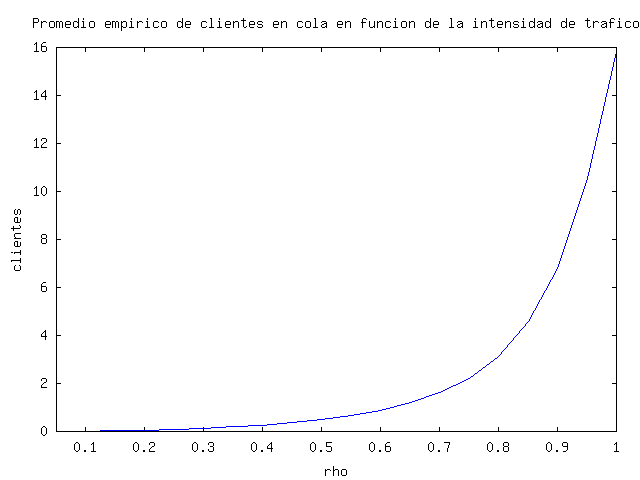
\includegraphics[width=8cm]{queueEmpiricVSrho}
\caption{\label{fig:meanQueue} Promedio emp\'irico de clientes en la cola en funci\'on de $\rho$}
\end{center}
\end{figure}

Se comparan los resultados obtenidos con el valor te\'orico de $L_q$ el cual se ense\~na en \eqref{eq:lQTheoretical}

\begin{equation}
\label{eq:lQTheoretical}
L_q = \dfrac{\rho^{2}}{1 - \rho}
\end{equation}

Los resultados de dicha comparacion se observan en la figura \ref{fig:meanQueueVS}. Se observa que ambas curvas
son casi id\'enticas salvo para los grandes valores de $\rho$ en los cuales se produce una diferencia dr\'astica.
Esto se debe a que para esos casos la simulaci\'on no finaliza al alcanzar un error menor al $5\%$ sino que finaliza
porque alcanza el tope m\'aximo de iteraciones a realizar ($2000$). \'Esto nos dice que para grandes valores de $\rho$
se hace m\'as dif\'icil lograr una buena aproximaci\'on al promedio de clientes en la cola.

\begin{figure}[ht]
\begin{center}
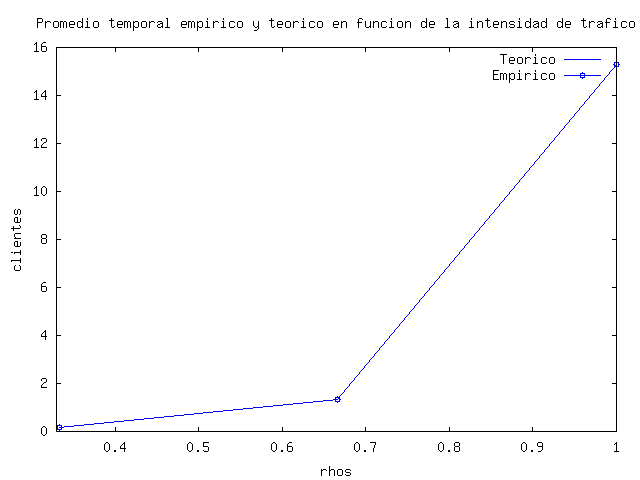
\includegraphics[width=8cm]{teoricoVSempirico}
\caption{\label{fig:meanQueueVS} Comparaci\'on del promedio emp\'irico y te\'orico de clientes en la cola en funci\'on de $\rho$}
\end{center}
\end{figure}

\newpage

\subsection{El tiempo est\'a de mi lado}
\label{sec:parte2}

La expresi\'on anal\'itica del tiempo medio de espera para un cliente que est\'a en una cola M/M/1 se define en \eqref{eq:wq}.
Por otra parte, la expresi\'on de su varianza se define en \eqref{eq:wqvar}.
Se puede ver la gr\'afica representada para 10 puntos en \ref{fig:teowq} donde
se ve claramente el comportamiento asint\'otico hacia el valor 1 (donde alcanza la singularidad).

\begin{equation}
\label{eq:wq}
  W_q = E (T_q)= \frac{1}{\mu-\lambda}
\end{equation}

\begin{equation}
\label{eq:wqvar}
  Var(T_q) = \frac{\rho(2-\rho)}{\mu^2(1-\rho^2)}
\end{equation}

Por otra parte, los resultados obtenidos emp\'iricamente de $W_q$ se pueden observar en \ref{fig:empwq}.
All\'a� vemos como para las 20 corridas de 200 simulaciones se aprecian los efectos de bordes finitos para
la proximidad al valor 1 (que tiene asociado 16 unidades de tiempo).
Una comparaci\'on de los dos resultados se puede observar m\'as claramente en \ref{fig:teovsempwq}.

A medida que las probabilidades de $\mu$ y de $\lambda$ convergen al mismo valor suceden varios fen\'omenos: 
\begin{enumerate}
\item Intuitivamente, la probabilidad que llegue un usuario $\lambda$ hace que lleguen usuarios casi a la misma velocidad que se van $\mu$. En este hipotético caso, esto se traduce en que el sistema a largo plazo se comiencen a acumular usuarios en la cola. Resultando en que no se llegue a dar abasto a atenderlos. Por lo que tiene sentido pensar que el tiempo de permanencia en la cola empiece a crecer.
\item Viendo el resultado anal\'i�tico se observar que la esperanza del tiempo en cola tiende a infinito al igual que su varianza. De esta forma, podemos concluir que el sistema se comportará de manera inestable. Si bien en la práctica no tiene sentido de hablar de tiempo infinito, se puede pensar como un colapso del servicio.
\item Como se mencion\'o anteriormente, el motivo por el cual en el gr\'afico \ref{fig:empwq} no se nota la divergencia es debido al efecto que se corrió un número finito de veces y con un número finito de personas. 
\item Cuando se acerca al valor de divergencia (o sea $\rho=1$), la f\'ormula \ref{eq:wqvar}  comienza a crecer.
Esto indica que cuanto mayor sea la diferencia entre $\mu$ y $\lambda$ (siempre que $\rho < 1$ porque sino eso
implicar\'i�a inestabilidad) mayor ser\'a la varianza.
Esto se traduce en que la esperanza tendr\'a menos volatilidad a medida que $\lambda$ sea mucho menor a $\mu$.
En un caso pr\'actico, nos asegura que si nuestro tiempo de servicio es bueno ser\'a probabil\'i�sticamente
insignificante la posibilidad de que el servicio se sature.
A medida que el servicio empeora, o se vuelve m\'as ineficiente, se somete a un mayor riesgo a ser saturado.


\end{enumerate}

\begin{figure}[ht]
\begin{center}
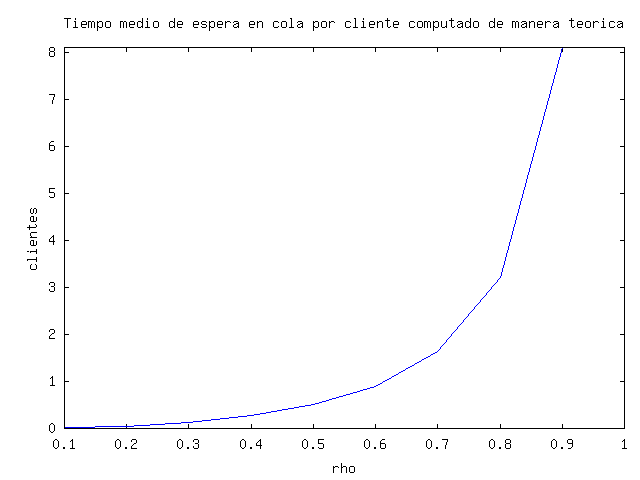
\includegraphics[width=8cm]{queueWaitTheoretical}
\caption{\label{fig:teowq} Tiempo de espera en cola te\'orico de los clientes en funci\'on de $\rho$}
\end{center}
\end{figure}
\begin{figure}[ht]
\begin{center}
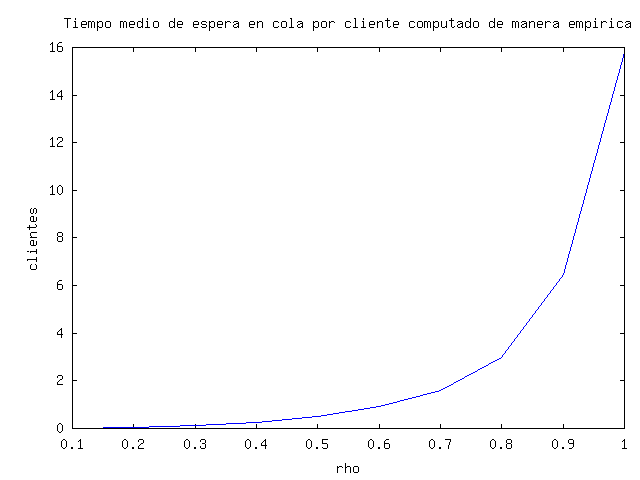
\includegraphics[width=8cm]{queueWaitEmpirical}
\caption{\label{fig:empwq} Tiempo de espera en cola empírico de los clientes en funci\'on de $\rho$}
\end{center}
\end{figure}
\begin{figure}[ht]
\begin{center}
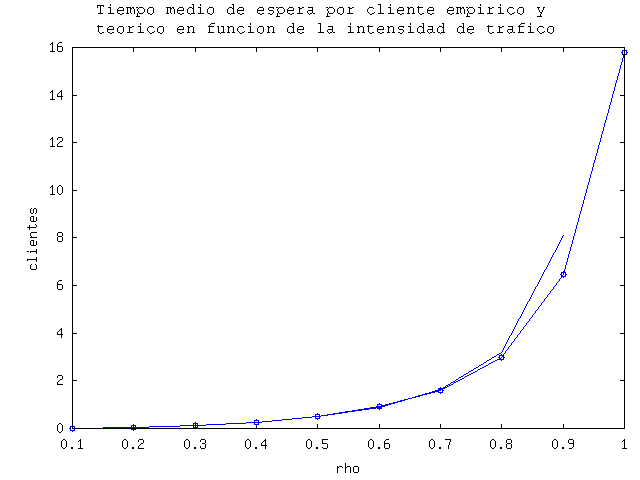
\includegraphics[width=8cm]{queueWaitCompare}
\caption{\label{fig:teovsempwq} Tiempo de espera en cola te\'orico y empírico de los clientes en funci\'on de $\rho$}
\end{center}
\end{figure}

\section{Inclusi\'on de un nuevo servidor}
\label{sec:mm2}

En esta secci\'on se introduce el uso de un sistema de colas M/M/2 (siguiendo la notaci\'on de Kendall)
con un esquema de 2 servidores atendiendo en paralelo y se quiere observar c\'omo la introducci\'on
de un nuevo servidor repercute en la longitud media de la cola. Para ello se utiliza el factor densidad de tr\'afico de clientes
\begin{equation}
\rho = \frac{\lambda}{\mu_{1} + \mu_{2}}
\end{equation}
para analizar la variaci\'on de la longitud media de la cola en funci\'on del mismo.
Debido a que este factor depende de 3 variables se fija $\lambda$ y se simplifica haciendo
$\mu_{1}=\mu_{2}$ y s\'olo se hace variar \'este \'ultimo par\'ametro.
A partir de simulaciones se obtiene la gr\'afica \ref{REF AL GRAFICO}. Si se observa {INCLUIR COMPARACION CON GRAFICO LOMBO}

\section{Resultados y Conclusiones}
\label{sec:conclusiones}
CONCLUIME

% TODO ver si corresponde
% \begin{thebibliography}{10}
% \bibitem{chiTable} Tabla $\chi^{2}$.
% \begin{verbatim}
% http://www.wiphala.net/research/manual/
% statistic/chi_cuadrado.html
% \end{verbatim}
% \bibitem{KSTable} Tabla Kolmogorov-Smirnov.
% \begin{verbatim}
% http://www.eridlc.com/onlinetextbook/
% appendix/table7.htm
% \end{verbatim} 
% \bibitem{TStudentTable} Tabla T Student. \begin{verbatim}www.elosiodelosantos.com/sergiman/archivos/tablat.xls\end{verbatim}
% \end{thebibliography}
\end{document}
